\section{Machine Learning}

\begin{definition}[\textit{Learning}]
    A computer program is said to learn from experience $E$ with respect to some class of tasks $T$ and performance measure $P$ if it improves with experience $E$. 
\end{definition}

Machine Learning derives knowledge from experience and induction.

In Machine Learning, we depend on computers to make informed decisions using new, unfamiliar data. 
Designing a comprehensive set of meaningful rules can prove to be exceedingly difficult. 
Machine Learning facilitates the automatic extraction of relevant insights from historical data and effectively applies them to new datasets.

The objective is to automate the programming process for computers, acknowledging the bottleneck presented by writing software.
Instead, our aim is to utilize the data itself to accomplish the required tasks.

\begin{figure}[H]
    \centering
    \begin{subfigure}{0.49\textwidth}
        \centering
        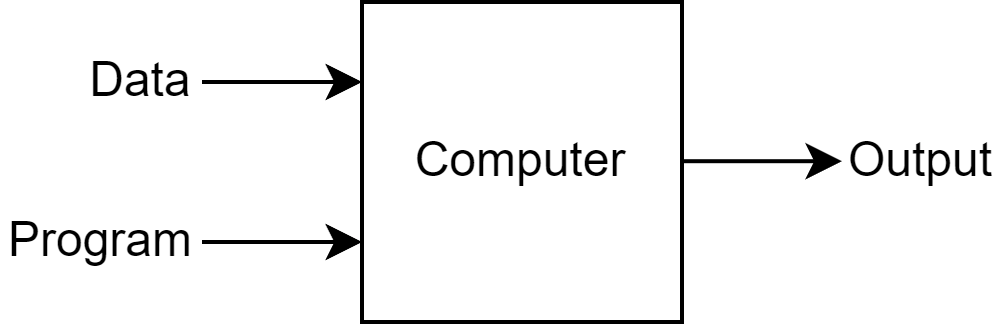
\includegraphics[width=0.9\linewidth]{images/program.png} 
        \caption{Programming}
    \end{subfigure}
    \begin{subfigure}{0.49\textwidth}
        \centering
        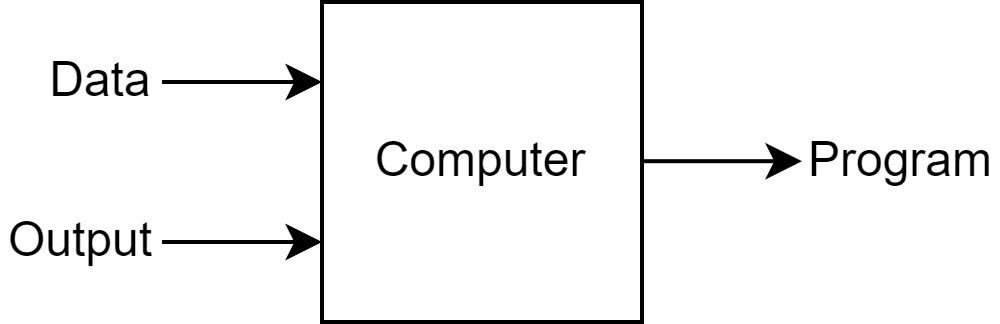
\includegraphics[width=0.9\linewidth]{images/learning.png}
        \caption{Machine Learning}
    \end{subfigure}
    \caption{Difference between programming and Machine Learning}
\end{figure}

Machine Learning paradigms can be categorized into three main types:
\begin{itemize}
    \item \textit{Supervised learning}: involves labeled data and direct feedback, aiming to predict outcomes or future events.
    \item \textit{Unsupervised learning}: operates without labeled data or feedback, focusing on discovering hidden structures within the data.
    \item \textit{Reinforcement learning}: centers around a decision-making process, incorporating a reward system to learn sequences of actions.
\end{itemize}

\subsection{Supervised learning}
Supervised learning encompasses several distinct tasks:
\begin{itemize}
    \item \textit{Classification}: this involves assigning predefined categories or labels to data points based on their features. 
        The model is trained on labeled data, learning patterns to predict the class labels of new data points.
    \item \textit{Regression}: the goal here is to predict continuous numerical values based on input features, as opposed to discrete class labels in classification. 
        The model learns a function mapping input features to output values.
    \item \textit{Probability estimation}: this task predicts the likelihood of certain events or outcomes occurring, often used to gauge the confidence of model predictions.
\end{itemize}
Formally, in supervised learning, a model learns from data to map known inputs to known outputs. 
The training set is denoted as $\mathcal{D}=\left\{\left\langle x,t \right\rangle\right\}$, where $t = f(x)$, with $f$ representing the unknown function to be determined using supervised learning techniques.

Various techniques can be employed for supervised learning, including linear models, artificial neural networks, support vector machines, and decision trees.

\subsection{Unsupervised learning}
Unsupervised learning encompasses two main tasks:
\begin{itemize}
    \item \textit{Clustering}: in this task, the objective is to group similar data points together based on their features, without predefined labels. 
        The goal is to uncover underlying patterns or structures within the data. 
        Clustering algorithms segment the data into clusters or groups, where data points within the same cluster exhibit greater similarity compared to those in different clusters. 
    \item \textit{Dimensionality reduction}: this task involves reducing the number of input variables or features in a dataset while retaining essential information. 
        This is often done to address the curse of dimensionality, enhance computational efficiency, and mitigate overfitting risks in models. 
        Dimensionality reduction techniques aim to transform high-dimensional data into a lower-dimensional representation while preserving most relevant information.
\end{itemize}
Formally, in unsupervised learning, computers learn previously unknown patterns and efficient data representations.
The training set is defined as $\mathcal{D}=\left\{ x \right\}$, where the goal is to find a function $f$ that extracts a representation or grouping of the data.

Various techniques are used for unsupervised learning, including k-means clustering, self-organizing maps, and principal component analysis.

\subsection{Reinforcement learning}
Reinforcement learning encompasses several key approaches:
\begin{itemize}
    \item \textit{Markov Decision Process}: a mathematical framework for modeling decision-making, involving states, actions, transition probabilities, and rewards. 
        The goal is to find a policy that maximizes cumulative rewards while considering uncertainty.
    \item \textit{Partially Observable MDP}: an extension of MDP where the current state is uncertain and must be inferred from observations. 
        The objective remains the same, but the agent maintains a belief over possible states based on observations.
    \item \textit{Stochastic games}: models for decision-making with multiple agents, where outcomes depend on actions and random factors. 
        Players aim to optimize strategies considering other players' actions and uncertainties.
\end{itemize}
In reinforcement learning, the computer learns the optimal policy based on a training set $\mathcal{D}$ containing tuples $\left\langle x,u,x^\prime,r \right\rangle$, where $x$ is the input, $u$ is the action, $x^\prime$ is the resulting state after the action, and $r$ is the reward.
The policy $Q^\ast$ is defined to maximize $Q^\ast(x,u)$ over actions $u$ for each state $x$ in the training set. 

Various techniques such as Q-learning, SARSA, and fitted Q-iteration are used to find this optimal policy.